\documentclass[aspectratio=169]{beamer}
%\documentclass[aspectratio=43]{beamer}
%\documentclass[handout]{beamer}

\graphicspath{{images}}
%%
%% Use my fancy hfd beamer template.
%%
\makeatletter
\def\input@path{{../hfd/}}
\makeatother
\usetheme{hfd}

%%
%% Some additional packages.
%%
\usepackage{lmodern}
\usepackage{pgfpages}
\usepackage{tabularx}
\usepackage{listings}
\usepackage{tikz}
\usetikzlibrary{arrows.meta, shapes.callouts, backgrounds}
\tikzset{
	notice/.style  = { fill=white, draw, rectangle callout, callout relative pointer={#1} },
}

% Code syntax highlighter
\usepackage{minted}

\usepackage[T1]{fontenc}

%%
%% Some beamer options.
%%
%\setbeameroption{hide notes} 							% Only slides
%\setbeameroption{show only notes} 						% Only notes
%\setbeameroption{show notes on second screen=right}	% Notes on the right
%%
%% include some general configuration that
%% remains constant for the whole lecture,
%% i.e., across all slide sets.
%%
\degree[B.Sc.]{Computer Science, B.Sc.}
\date[2024]{WiSe 2024/25}
\title[DS]{Distributed Systems}
\subtitle[Introduction]{Lecture 01: Introduction}
\author[Christoph König]{Prof. Dr.-Ing. Christoph König}

%%
%% Define some variables.
%%
\newcommand{\moodlelink}{https://lernen.hs-fulda.de/course/view.php?id=20980}
\newcommand{\moodlecourseid}{Verteilte Systeme - AI1015 (WiSe24/25)}

\subtitle[TIME]{Lecture 14: Time in Distributed Systems}

%%
%% Let's start.
%%
\begin{document}


%%
%% Title page.
%%
\begin{frame}
	\titlepage
\end{frame}

%%
%%

%%
%%
\begin{frame}{Outline}
    \begin{minipage}[t]{0.65\textwidth}
        \begin{itemize}
            \item Challenges in distributed systems
            \begin{itemize}
                \item Consistency
                \item Concurrency
            \end{itemize}
            \item Physical and logical time
            \begin{itemize}
                \item … and how to distribute it
            \end{itemize}
            \item Time synchronization
            \begin{itemize}
                \item Skew and drift
                \item Cristian's algorithm
                \item Berkeley algorithm
                \item NTP and PTP
            \end{itemize}
            \item Logical clocks
            \begin{itemize}
                \item Relations
                \item Lamport clock
                \item Vector clock
            \end{itemize}
        \end{itemize}
    \end{minipage}
    \begin{tikzpicture}[remember picture, overlay]
        \node[anchor=south east, xshift=-0.5cm, yshift=0.5cm]
            at (current page.south east)
        {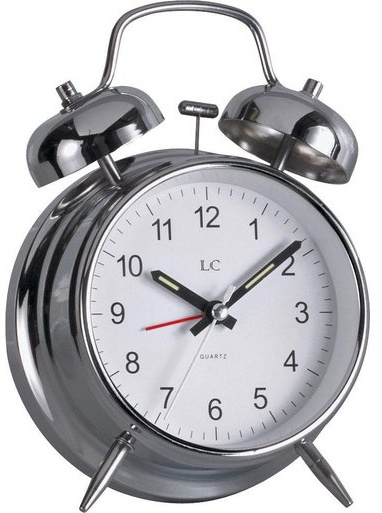
\includegraphics[width=3.5cm]{slide2.jpg}};
    \end{tikzpicture}
\end{frame}
%%
%%

\begin{frame}{Synchronization and drift}
      \begin{minipage}[t]{0.80\textwidth}
        \begin{itemize}
          \item Goal: All hosts should have the same time
          \item Challenges
            \begin{itemize}
                \item Clocks can have different start times
                    \begin{itemize}
                        \item $t_{\text{clock\_a}} \neq t_{\text{clock\_b}}$
                        \item Called \textbf{skew}
                    \end{itemize}
                \item Clocks can run at different speeds
                    \begin{itemize}
                        \item Called \textbf{drift}
                        \item Ideal: $dC/dt = 1$
                    \end{itemize}
            \end{itemize}
            \item Drift example
                \begin{itemize}
                    \item Let $p = \text{the maximum deviation}$\\
                    e.g., given by the manufacturer, such that\\
                    $1 - p \leq \frac{dC}{dt} \leq 1 + p$
                    \item Question: What is the maximum difference of two drifting clocks after $\Delta t$ time units?
                    \item Answer: $2p \Delta t$
                \end{itemize}
        \end{itemize}
      \end{minipage}
        %% Graph
        \begin{tikzpicture}[remember picture, overlay]
      \node[anchor=north east, xshift=-0.5cm, yshift=-1.5cm] at (current page.north east) {
        \begin{tikzpicture}[>=Latex, scale=1]
          
          % Axes
          \draw[thick,->] (0,0) -- (0,3.2) node[anchor=east] {Clock time C};
          \draw[thick,->] (0,0) -- (3.6,0) node[anchor=north] {UTC t};
    
          % Clock line length
          \def\L{4.2}
    
          % Ideal clock (slope = 1)
          \draw[thick, green!70] (0,0) -- ({\L*cos(45)}, {\L*sin(45)})
            node[pos=0.7, sloped, above, text=green!50!black]{\scriptsize Ideal clock};
    
          % Fast clock (steeper)
          \draw[dashed, red, thick] (0,0) -- ({\L*cos(60)}, {\L*sin(60)})
            node[pos=0.7, sloped, above, text=red]{\scriptsize Fast clock};
    
          % Slow clock (flatter, shorter dashes)
          \draw[dash pattern=on 2pt off 1pt, red, thick] (0,0) -- ({\L*cos(30)}, {\L*sin(30)})
            node[pos=0.7, sloped, above, text=red]{\scriptsize Slow clock};
    
          % Slope labels
          \node[anchor=west] at ({\L*cos(60)}, {\L*sin(60)}) {\scriptsize $\frac{dC}{dt} > 1$};
          \node[anchor=west] at ({\L*cos(45)}, {\L*sin(45)}) {\scriptsize $\frac{dC}{dt} = 1$};
          \node[anchor=west] at ({\L*cos(30)}, {\L*sin(30)}) {\scriptsize $\frac{dC}{dt} < 1$};
    
        \end{tikzpicture}
      };
    \end{tikzpicture}
\end{frame}
%%
%%
%%
\begin{frame}{Message delays (cont’d)}

  \begin{itemize}
    \item How to get (and calculate) message delays?
  \end{itemize}

  \begin{center}
  \begin{tikzpicture}[>=Stealth, node distance=2cm, every node/.style={font=\scriptsize}]
    % Client and Server labels
    \node at (-0.7,1) {
\includegraphics[width=0.9cm]{client.jpg}};
    \node at (-0.7,2.5) {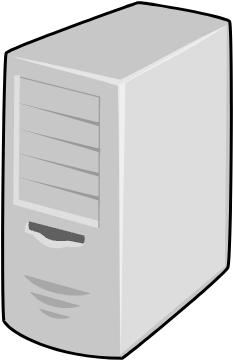
\includegraphics[width=0.7cm]{server.jpg}};
    \node at (-1.6,2.5) {\scriptsize Server};
    \node at (-1.6,1) {\scriptsize Client};

    % Timeline lines
    \draw[->,thick] (0,2.5) -- (5,2.5) node[right] {\scriptsize time};
    \draw[->,thick] (0,1) -- (5,1) node[right] {\scriptsize time};

    % Events
    \filldraw[blue!70] (1,1) circle (3pt) node[below] {$t_0$};
    \filldraw[blue!70] (2,2.5) circle (3pt) node[above] {$t_1$};
    \filldraw[blue!70] (3.5,2.5) circle (3pt) node[above] {$t_2$};
    \filldraw[blue!70] (4,1) circle (3pt) node[below] {$t_3$};

    % Arrows for messages
    \draw[->,thick] (1,1.1) -- (1.9,2.4);
    \draw[->,thick] (3.5,2.4) -- (4,1.1);
  \end{tikzpicture}
  \end{center}

  \begin{itemize}
    \item Approximation
    \[
      OWD_{\text{approx}} = \frac{t_3 - t_0 - (t_2 - t_1)}{2}
    \]
    \item Question: What is the maximum error?
  \end{itemize}

\end{frame}
%%
%%
\end{document}